\documentclass[onecolumn, draftclsnofoot,10pt, compsoc]{IEEEtran}
\usepackage{graphicx}
\usepackage{url}
\usepackage{setspace}
\usepackage{csquotes}
\usepackage{float}

\usepackage{geometry}
\geometry{textheight=9.5in, textwidth=7in}

% 1. Fill in these details
\def \CapstoneTeamName{	Short Circuit Comedy Club	}
\def \CapstoneTeamNumber{		CS13}
\def \GroupMemberOne{			Kevin Talik}
\def \GroupMemberTwo{			Arthur Shing}
\def \GroupMemberThree{			Anish Asrani}
\def \CapstoneProjectName{		How to Build an Effective Robot Comedian}
\def \CapstoneSponsorCompany{	Oregon State University}
\def \CapstoneSponsorPerson{		Dr. Heather Knight}

% 2. Uncomment the appropriate line below so that the document type works
\def \DocType{		%Problem Statement
				%Requirements Document
				%Technology Review
				%Design Document
				Progress Report
				}
			
\newcommand{\NameSigPair}[1]{\par
\makebox[2.75in][r]{#1} \hfil 	\makebox[3.25in]{\makebox[2.25in]{\hrulefill} \hfill		\makebox[.75in]{\hrulefill}}
\par\vspace{-12pt} \textit{\tiny\noindent
\makebox[2.75in]{} \hfil		\makebox[3.25in]{\makebox[2.25in][r]{Signature} \hfill	\makebox[.75in][r]{Date}}}}
% 3. If the document is not to be signed, uncomment the RENEWcommand below
%\renewcommand{\NameSigPair}[1]{#1}

%%%%%%%%%%%%%%%%%%%%%%%%%%%%%%%%%%%%%%%
\begin{document}
\begin{titlepage}
    \pagenumbering{gobble}
    \begin{singlespace}
 %   	\includegraphics[height=4cm]{coe_v_spot1}
        \hfill 
        % 4. If you have a logo, use this includegraphics command to put it on the coversheet.
        %\includegraphics[height=4cm]{CompanyLogo}   
        \par\vspace{.2in}
        \centering
        \scshape{
            \huge CS Capstone \DocType \par
            {\large\today}\par
            \vspace{.5in}
            \textbf{\Huge\CapstoneProjectName}\par
            \vfill
            {\large Prepared for}\par
            \Huge \CapstoneSponsorCompany\par
            \vspace{5pt}
            {\large Prepared by }\par
            Group\CapstoneTeamNumber\par
            % 5. comment out the line below this one if you do not wish to name your team
            \CapstoneTeamName\par 
            \vspace{5pt}
            \vspace{20pt}
        }
        \begin{abstract}
  	     % 6. Fill in your abstract    
			The purpose of this document is to outline the research papers that this team will create to conclude during Spring Term 2018. 
			The three members of the \textit{Short Circut Comedy Club} have spent their time during winter term perfomring research under Dr. Heather Knight at Oregon State University.
			The focus of this project is to study the effect a robot comedian can have on a crowd of humans.
			Kevin Talik's research has been spent understanding what a Comedian can do to "Adapt" to a performance. 
			Arthur Shing has been studying the voice of the robot, and the difference between "Robot and Human" character.
			One final aspect of Stand-Up Comedy that we studied is "Crowd Work". Anish Asrani has spent most of his time developing spontaneous Crowd-Interactions during the set.
        \end{abstract}     
    \end{singlespace}
\end{titlepage}
\newpage
\pagenumbering{arabic}
\tableofcontents
% 7. uncomment this (if applicable). Consider adding a page break.
%\listoffigures
%\listoftables
\clearpage

% 8. now you write!
\section{Overview}
	This paper will have three separate sections written by each respective member of the \textit{Short Circut Comedy Club}. 
Each section will be prefaced with a summary of the work that has been done during the first five weeks of Spring Term.


Our largest problem that has been impeding our progress is Audience Sensing. 
We had intended to use only microphones for the sensing, however after testing, we realized that the background sound of a room can vary so much that using \textit{only} the microphone is unreliable.

Since we had reached our 1.0 requirements for our software, we have been investigating how to make our performance \textit{Coherent}. Kevin Talik has sinched down his "Mechanical Engineering hat" and started developing controllers for the crowd to interface with the show. If the robot can cross-reference the sound of the room with the input of the controllers, the robot can reason a more viable response from the humans. This is similar to how autonomous cars cross-reference infared imaging with radar imaging to detect different objects. Giving the robot more "senses" will hopefully aide in the success of the performance.

Arthur Shing has spent a heavy amount of time writing parallel jokes between topics to test research categories. We hope that another team will be able to pick up our work after we leave this term, and we need to be able to have many of variants of our jokes to test the delivery of different jokes across different "topics".

Another large problem with our performance is \textit{Coherence}. If people cannot hear, or understand what the robot is trying to do, the audience often misses the punch of the joke.
This makes setting up a premise of a joke fail, leaving the human in a state of confusion. The jokes we have written are clean, simple, and stupid. If a human misses one \textit{state} of the current running behavior, the joke fails for the human.
Anish Asrani has been working on transitioning in between jokes, and getting the audience interacting with the robot before the bot starts telling a joke.

Concluding this document will be a section expanding the tasks that need to be done before the Expo. We ideally have more time to write our research papers after the big event, and will be spending our time perfecting our performance before showing humans the system.

\section{Adapation}
\subsection{Summary of Work Done}
 This section is written by Kevin Talik. I have been developing controllers and working closely with our TA, Behnam Saeedi. Additionally, I have been working meticulously with my team to make our systems work together. Similar to physical systems, virtual systems need to be able to be comprehensible to one human in order to make the system "human-readable".

 One human needs to be able to descend into the command line, armed with documentation, and be able to understand the code in a few moments. If a reader of a text file \textit{cannot} understand the code after a few minutes of scanning the document, it is the responsibility of the writer to make the document comprehensible.
 \subsection{Synopsis of Weekly Blog Posts}

 \subsection{Week 1} I met with Heather, and discussed why I got a B for the last term. I was able to explain the team dynamics of creating software with three different people working in different directions. If you make machines alone, you make machines that work alone. All of my work was virtual, and she never looked at my code for either the \textit{Haiku Bot} that I made, or the virtual \textit{Bayesian Network} implementation of our jokes Additionally, I could never get my team to use the scripting tools to insert jokes into a pickle library.

Winter term, we spent so much time apart, that while we all me the requirements for 1.0, we had a bunch of things that were not being tested together. I told Heather that I started performing stand-up comedy, and went to two open mic events at bombs away during winter term.

Since all of our requirements were met, I started to get creative and mechanical about how we could solve some of the problems with our robot comedian. Another problem is communication, and using the same Reference of Language during our team meetings.

I have been talking to Heather about the "Mythical Man Month", and how there is No Silver Bullet to software engineering. We needed to made a design document to flesh out the details of software so that the expectation is understood. When my client edited my portions of my design document without my conformation, I was unaware of the software that she expected me to make. Even though I thought I had made it, my client did not.

\subsection{Week 2} "Using machines as an end to means, not a means to an end." Robots can switch context impeccably fast, and cannot be trusted the same way a human can be trusted. Experiences for humans have value for the human, where the only value we put on the jokes are the one we, as humans and comedians, value.

\subsection{Week 3} I realized that I know nothing about building mechanical machines. Anish and I went to Hweekend and I finally learned the difference between a volt, watt and amp (please don't hurt me).

\subsection{Week 4} TCP server works on the controller, and it can send commands to the NAO. I think this is beta functionality for the controller.

\subsection{Week 5} I finished my final design of the controller, and I want to make an image to put onto the RPIs, so that when they fail during expo, we can reflash the units quickly. We also did the maker fare this last weekend, and we got crazy feedback about how to make our controllers better. Decided to just run with a two button design, instead of three. It will be easier to explain branching between two options over three. Kids stop listening when you put a controller in their hands.

\subsection{Outline of Research Paper}
	I have been sharing my sources with Kirsten personally for the paper this term, and will work harder on compiling our bibliography into one document. I want to structure this paper equally with science fiction sources as well as non-fiction sources for the "gap" we are researching. Using research from Judy Goldsmith, studying the effects of "Science Fiction as an Introduction to AI Research", I believe that using fictional comparisons to actual machines that humans are making is a brilliant way to discuss the ethical implications of AI. People have been describing machines that are being currently built; in 2018, humans have the resources to physically build these theoretical machines.

	Moore's law has slowed down, and it may be because humans do not have a deterministic amount of time to solve software problems. Robots can reduce in constant time (check out the Complete Fair Scheduler in the Linux Kernel), and can reduce NP-Hard problems faster than humans can. If we can find a way to make humans learn as fast as robots, humans can still work on software problems.

	The technology I am using to describe our robot is the \textit{Talbot Yancy} Robot and the \textit{Rhetorizor} from \textit{"The Penultimate Truth"} (The tech is mentioned in the first chapter, however, it is used heavily throughout the book). I want to thoroughly discuss the difference between making a robot a robot comedian, and how it is \textit{substantially} different than making a comedian a robot comedian. What I always say to myself while making AI is "use machines as an end to means, and people as a end through means." This is a basis of my paper, following a discussion of being able to trust a machine that can make you laugh (you shouldn't). Google the "Paglacio the Clown" joke, from "The Watchmen".

\subsection{Concluding Thoughts}
 I want to get a working bibliography file for our whole team to use. This will allow us to work together using the same resources. When we write a final document, having reasonable bibliographies will make finishing and publishing this paper a breeze.


 Also, I need to find a quote for the paper. Here is the one I want to use:


 \begin{displayquote}
	 "You're growing, learning so quickly. I am frightened of what you might become, what path you might take."
	 -Bernard Lowe, \textit{Westworld, Season 2, Episode 1}
 \end{displayquote}



\section{Crowd-work}
This section will discuss the crowd-work portion of the project. It is written by Anish Asrani. To recap, crowd-work is essentially interacting with the audience to integrate them into the performance. It is a medium to connect with the audience and could help the audience enhance their perceptions about the robot. The robot has a handful of sensors that are vital to this aspect of crowd interactions. 

\subsection{Summary of Work Done}
A lot of time this term was spent refining our system and planning for failure and testing those systems out with an audience. Like Kevin mentioned earlier, the controller was put in place for situations when it is not feasible for the robot to listen to the audience. I was working on basic TCP communication script that launches a roboy behavior on the robot directly from the controller.  Also, in other situations, if the audience participant does not respond to the robot/the robot does not get any input, the robot will move forward with the comedy set rather than wait for that input. 

We participated in HWeekend and Corvallis Maker Fair to put our project out there and get some feedback for the comedy sets we have implemented. We got an idea of which jokes work and do not work with the audience, how to refine the timing of the joke so the audience does not miss the punch line, and situations where we need to have a backup. Both of these events were really helpful to actually understand how to work the robot in various audience settings and also got an idea of things that can go wrong. 

In situations where the robot does not hear what the audience says or does not get any feedback - there are two backup options that I have worked on depending on the specific behavior. One of them waits for a pre-defined period of time for input before moving on with the script (and potentially acknowledging the lack of input from the audience). Another one is to skip certain behaviors on tapping one of the various tactile sensors on the robot (3 on the head, one on each foot and arm).

One of the scripts that I tested a lot during the Corvallis Maker Fair involved asking the audience questions about a specific topic, make a few comments about it, and then phase into a joke about that specific topic (e.g. dating as a topic in this case). People seemed to enjoy that since it did not abruptly throw a random topic at them, it made them think about it which helped make the joke relatable. 

\subsection{Left To Do}
All of the functionality and systems on the robot are already in place. It's just a matter of mixing and matching various behaviors to figure out the optimal set when demoing to people at the Expo. Apart from that, we need to optimize the controller functionality to properly communicate with the robot. We will also use the observations of people's reactions from the events we attended (including Expo) as preliminary results for the research paper. 

\subsection{Problems}
The volume levels on the robot is one major issue. People need to really focus on the robot's audio to understand it sometimes as well as the robot looking for audio input. This became very evident during Corvallis Maker Fair when it was fairly loud all around. So in situations where we anticipate loud noises (e.g. Atrium area during Expo), keeping the robot's dialog simple and focusing more on animation and movement would be the right idea. However, this would only affect about half of our time during the Expo since we will have a classroom where we can have shows in a quieter environment. 

\begin{figure}[H]
  \centering
  \includegraphics[width=0.75\textwidth,height=0.75\textheight,keepaspectratio]{comedy-1.png}
  \caption{People leaning in to listen to Ginger}
	\label{fig:comedy-1}
\end{figure}

One issue that came up during HWeekend was that the face detection freaked out when there were multiple faces and sounds from the audience. I added some conditions for number of faces (as well as the timer system mentioned earlier) that fixed the issue and it worked successfully during Corvallis Maker Fair. Fixing issues like is where exposure to real audience really helped.

In situations like Maker Fair where it was \textit{fair}ly loud, I had to improvise and I decided to use the Choregraphe emulator as a backup. I put my laptop screen with the emulator (shown in Fig 2) behind the robot, so people could read it as they go. This seemed to help a lot. While it is not perfect and can distract people away from the robot, it was a decent way to get our jokes across in an unfavorable environment.

\begin{figure}[H]
  \centering
  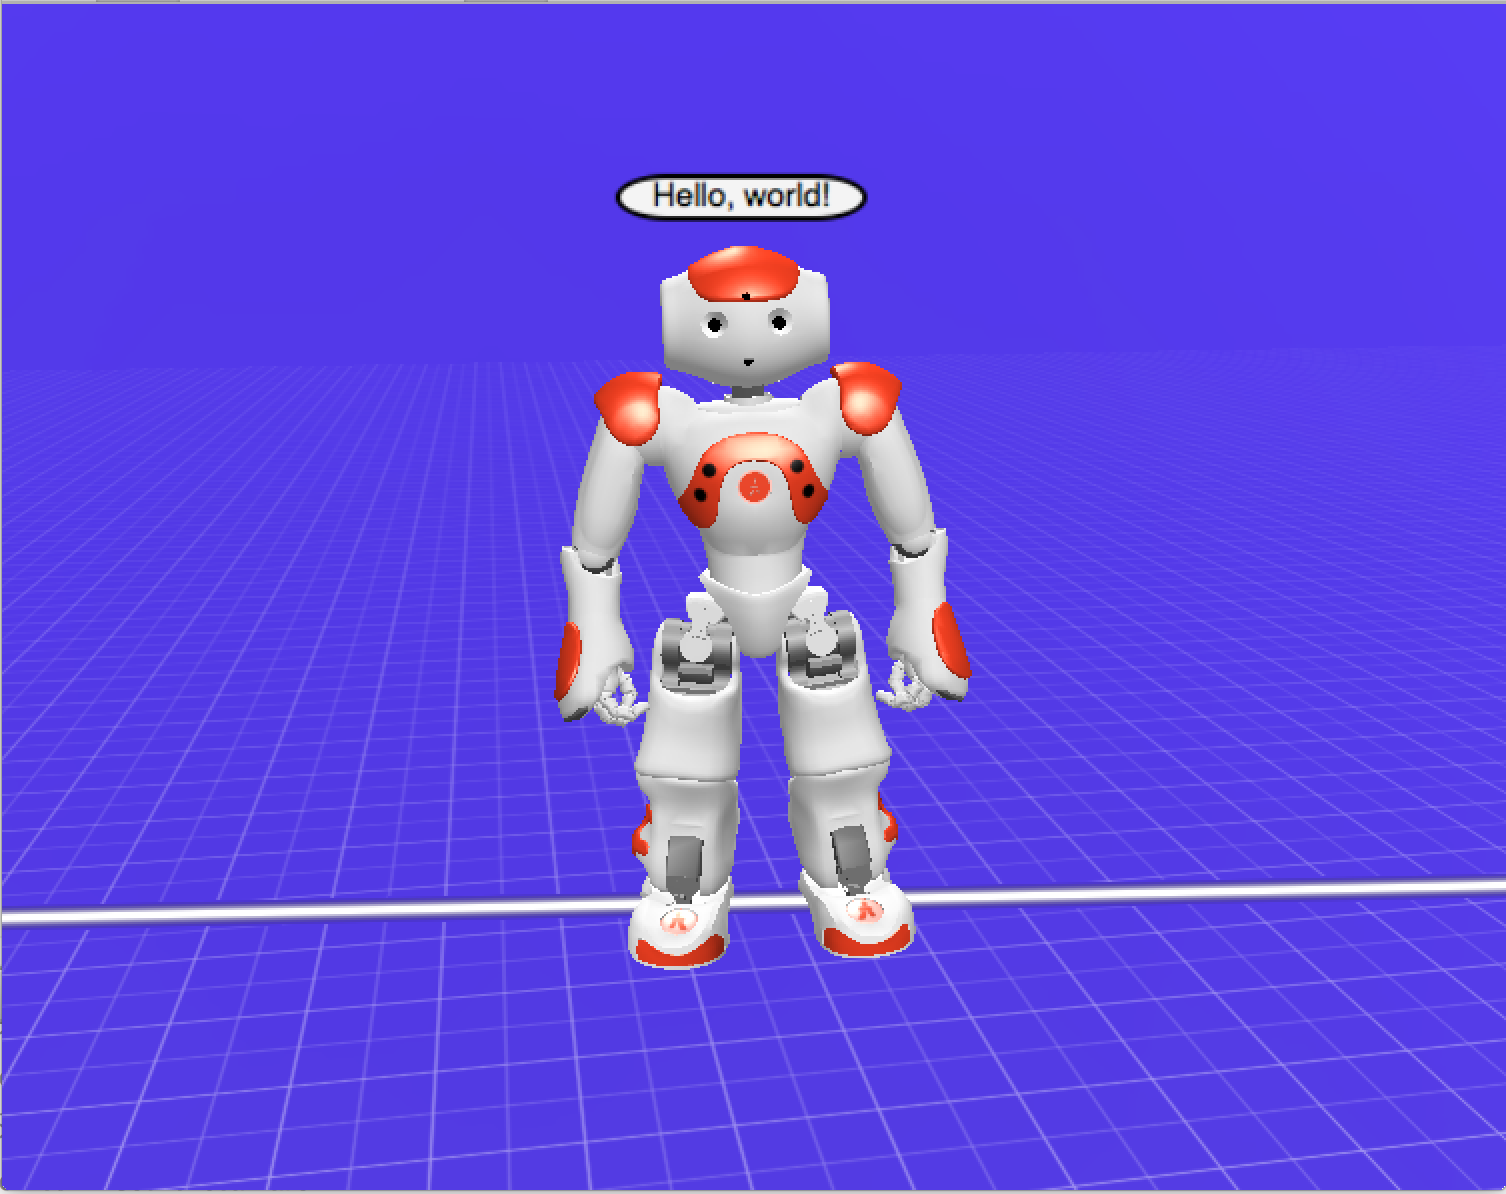
\includegraphics[width=0.75\textwidth,height=0.75\textheight,keepaspectratio]{comedy-2.png}
  \caption{Choregraphe emulator with subtitles}
	\label{fig:comedy-2}
\end{figure}

\subsection{Outline of Research Paper}
In my research paper, I will be discussing the importance of crowd-work for a robot performing comedy. The aspects of crowd-work were: (1) No crowd-work (2) Fake crowd-work (3) Real crowd-work. The first part involves not acknowledging the audience at all. The second is making educated guesses about the audience demographic and using that to make comments. The final one is real crowd-work where the robot uses the in-built sensors to listen to the audience.

From the performances we have had so far, I hypothesize that crowd-work does not matter initially. The sheer novelty of the robot telling jokes is enough to fascinate the audience and pull them in. Crowd-work starts to matter after the audience has already heard a couple jokes. Using those spontaneous interactions when the audience's fascination is about to wear off throws them off and breaks their expectations. It adds a new layer of comedy that the audience did not expect at first. Obviously, our sample spaces are not the biggest and this is just a theory that would require further testing; testing during Expo and beyond. 

\subsection{Concluding Thoughts}
Overall, the project is coming together pretty well. We have preliminary observations for the research. We need to optimize our sets for Expo using those observations to try and get better reception at the Expo. 

\section{Final Tasks for Spring Term Progress}

\end{document}
